\documentclass{article}
\usepackage{iclr2027_conference,times}
\usepackage{amsmath,amssymb,mathtools}
\usepackage{graphicx}
\usepackage{booktabs}
\usepackage{array}
\usepackage{xcolor}
\usepackage{hyperref}
\usepackage{url}
\usepackage{enumitem}
\usepackage{microtype}
\hypersetup{hidelinks}
\setlength{\emergencystretch}{2em}

\newcommand{\TC}{\textsc{TaskCognition}}
\newcommand{\D}{\ensuremath{\mathrm{D}}}
\newcommand{\Rpol}{\ensuremath{\mathrm{R}}}
\newcommand{\1}{\mathbb{I}}
\newcommand{\E}{\mathbb{E}}
\newcommand{\Ew}{\mathbb{E}_{w}}
\newcommand{\Prb}{\mathbb{P}}
\newcommand{\NA}{\textemdash}
\newcommand{\hInd}{h_{\mathrm{ind}}}
\newcommand{\Rspoil}{R_{\mathrm{spoil}}}

\title{TaskCognition: When Does Overuse of Reasoning Models Degrade Answer Performance?}
\author{Anonymous authors\\Paper under double-blind review}
% Do not uncomment for anonymous review.
% \iclrfinalcopy

\begin{document}
\maketitle

\begin{abstract}
We propose \TC{}, a pre-results protocol for choosing between exactly two fixed inference packages on one frozen Qwen3-8B checkpoint: direct answering (\D) and bounded native thinking (\Rpol). Exactly one input-only gate acts before generation, and deployment makes exactly one answer call. The empirical question is whether supervision on direct-relative native-score benefit and package-relative independent-draw perfect-to-imperfect spoilage improves constrained deployment over same-resource winner and factorized outcome routers. A disjoint development stage freezes both packages before final labels; separate train, tune, held-out audit, and test splits then have immutable roles. Each learned method selects one candidate on tuning data and receives its own finite-sample empirical-Bernstein audit of score, cost, spoilage, and denominator adequacy. Audit failure forces direct deployment. Confirmatory evaluation requires test-set improvement over always-direct, winner, and factorized deployments. The audit is a deployment safeguard, not a new risk-control method. No TaskCognition experiment, power study, audit, or test has been run, and all result cells are empty.
\end{abstract}

\section{Introduction}
Reasoning traces can improve multi-step problem solving \citep{wei2022chain}, but a longer or explicit process is costly and may reduce performance in particular settings \citep{pmlr-v267-liu25t,wu2026more,srivastava-etal-2026-llms}. This motivates a concrete deployment question: before any answer is generated, when should a system use a bounded native-thinking package rather than a direct package?

\paragraph{Scope.}
We compare two named inference packages on one checkpoint, not latent cognition and not the causal effect of exposing a rationale. In the title, \emph{overuse} is policy-relative shorthand for sending an input to \Rpol{} when the declared score--cost--spoilage objective would prefer \D. It neither attributes excessive internal cognition to the model nor claims that reasoning models generally degrade performance. Exactly one learned input-only, pre-generation gate observes the query; deployment invokes exactly one of \D{} and \Rpol{} once. Tools, agents, additional checkpoints, post-answer switching, and deployable cascades are outside scope.

Routing itself is established \citep{pan-etal-2024-dynathink,zhou2026select,zhang2025synapseroute,guo2026think,wang2025semantic,pan2025route}. Our proposed contribution is instead an empirical comparison: does learning direct-relative paired benefit together with independent-draw perfect-to-imperfect spoilage improve constrained deployment beyond an equally resourced winner router and an equally resourced factorized outcome router? The held-out audit merely safeguards deployment of a tune-frozen candidate. It is not the statistical novelty. A null comparison, frequent fallback, or infeasible package is a valid outcome rather than permission to add policies.

\section{Related Work and Claim Boundary}
\paragraph{Routing and adaptive effort.}
Select-then-Solve, DynaThink, SynapseRoute, Think When Needed, When to Reason, and Route to Reason allocate inference regimes before or during generation \citep{zhou2026select,pan-etal-2024-dynathink,zhang2025synapseroute,guo2026think,wang2025semantic,pan2025route}. Broader methods allocate planning or decomposition \citep{yang2026ares,paglieri2025learning,liu-etal-2025-select-decompose,prasad-etal-2024-adapt}. \TC{} is a narrow algorithm-selection study \citep{rice1975algorithm}; its value must come from the preregistered comparison, not a configuration-only novelty claim.

\paragraph{Cascades and risk control.}
Confidence cascades observe a realized direct preview before escalating \citep{lu2025prolonged,lewislim2026confidence}; that information set induces a distinct preview-conditional risk. Cascades are therefore excluded from the primary comparison and may appear only in a secondary future analysis that charges the preview and defines a separate estimand. Conformal Risk Control, Conformal Thinking, and Learn then Test motivate explicit post-selection risk accounting \citep{angelopoulos2024conformal,wang2026conformal,angelopoulos2025learn}. Our fixed-candidate audit is not any of those procedures and provides no conformal or distribution-free guarantee.

\paragraph{Reasoning degradation.}
Mind Your Step, When More Is Less, and LLMThinkBench already motivate broad degradation questions \citep{pmlr-v267-liu25t,wu2026more,srivastava-etal-2026-llms}. Any eventual result here remains checkpoint-, package-, scorer-, cap-, and distribution-relative. Audit passage only authorizes one frozen deployment rule.

\section{Estimands and Constrained Objective}
Let $F\in\{1,\ldots,6\}$ denote a prespecified Reasoning Gym family. Every primary tuning, audit, and test quantity uses
\begin{equation}
 \Ew[T]=\frac{1}{6}\sum_{f=1}^{6}\E[T\mid F=f].
 \label{eq:ew}
\end{equation}
For input $X=x$, independent package draws yield native scores $S_a^{(1)}\in[0,1]$ and perfect-correctness indicators $Y_a^{(1)}=\1\{S_a^{(1)}=1\}$, $a\in\{\D,\Rpol\}$. Write $p_a(x)=\Prb(Y_a^{(1)}=1\mid X=x)$ and
\begin{equation}
 \hInd(x)=\Prb\{Y_\D^{(1)}=1,Y_\Rpol^{(1)}=0\mid X=x\}
 =p_\D(x)\{1-p_\Rpol(x)\}.
 \label{eq:hind}
\end{equation}
This is \emph{package-relative independent-draw perfect-to-imperfect spoilage}. It is neither a same-seed flip nor a causal statement about switching an already-correct answer. A gate $g(X)\in\{0,1\}$ routes to \Rpol{} when $g=1$. Its aggregate risk is
\begin{equation}
 \Rspoil(g)=\frac{\Ew[g(X)\hInd(X)]}{\Ew[g(X)p_\D(X)]},
 \label{eq:rspoil}
\end{equation}
when the denominator is positive.

A direct redraw can disagree even without changing packages. We therefore report, descriptively,
\begin{align}
 h_{DD}(x)&=p_\D(x)\{1-p_\D(x)\},\\
 R_{DD}(g)&=\frac{\Ew[g(X)h_{DD}(X)]}{\Ew[g(X)p_\D(X)]},\\
 \Delta_{DD}(g)&=\Rspoil(g)-R_{DD}(g)
 =\frac{\Ew[g p_\D(p_\D-p_\Rpol)]}{\Ew[g p_\D]}.
 \label{eq:hdd}
\end{align}
These are direct--direct independent-redraw references only; they neither replace Eq.~\ref{eq:rspoil} nor define a causal excess. For partial scores, another descriptive quantity is
\begin{equation}
 d_\epsilon(x)=\Prb\{S_\D^{(1)}-S_\Rpol^{(1)}\geq\epsilon\mid X=x\},
 \quad \epsilon\in\{0.10,0.25\}.
 \label{eq:degrade}
\end{equation}
We will report all-input and routed-subset aggregates. Expected score change and $d_\epsilon$ complement perfect-to-imperfect spoilage but do not enter its primary constraint.

For $K\geq2$ draws per package and input $i$, the prespecified finite-$K$ estimators are
\begin{align}
 \widehat p_{ai}&=K^{-1}\sum_{k=1}^{K}Y_{aik},\qquad
 \widehat h_{\mathrm{ind},i}=\widehat p_{\D i}(1-\widehat p_{\Rpol i}),\\
 \widehat h_{DD,i}&=\frac{K}{K-1}\widehat p_{\D i}(1-\widehat p_{\D i}),\qquad
 \widehat d_{\epsilon,i}=K^{-2}\sum_{k,\ell}\1\{S_{\D ik}-S_{\Rpol i\ell}\geq\epsilon\}.
 \label{eq:finitek}
\end{align}
The direct and reasoning draw sets are conditionally independent, making $\widehat h_{\mathrm{ind},i}$ unbiased for Eq.~\ref{eq:hind}; $\widehat h_{DD,i}$ is the distinct-draw order-two U-statistic \citep{hoeffding1948class}. The cross-products overlap. Neither $K^2$ cross-package cells nor $K(K-1)$ direct pairs are independent observations: the complete input cluster is the inferential unit.

Let $S_g=(1-g)S_\D+gS_\Rpol$. The restricted decision family is tuned for
\begin{equation}
 \max_{g\in\mathcal G}\ \Ew[S_g]
 \quad\text{s.t.}\quad \Ew[C_g]\leq\beta,
 \qquad \Rspoil(g)\leq\alpha.
 \label{eq:objective}
\end{equation}
Development fixes one scalar, nonduplicative resource ledger: either a monetary token/call schedule or hardware service time, but not both charged for the same serving work. Calls, tokens, latency, hardware, batching, concurrency, caching, and warm-up remain separate descriptive fields. Let $c_\D^{\rm ref},c_\Rpol^{\rm ref}$ be development reference package charges. The common exogenous budget is frozen before tuning as
\begin{equation}
 \beta=c_\D^{\rm ref}+\rho(c_\Rpol^{\rm ref}-c_\D^{\rm ref}),\qquad \rho=1/2.
 \label{eq:beta}
\end{equation}
Every method is assessed against this same $\beta$. Its own gate, any declared preview, every dispatched pre-admission retry, and the selected answer are charged exactly once; its gate cannot expand $\beta$.

\section{TaskCognition and Learning Targets}
\begin{figure}[t]
 \centering
 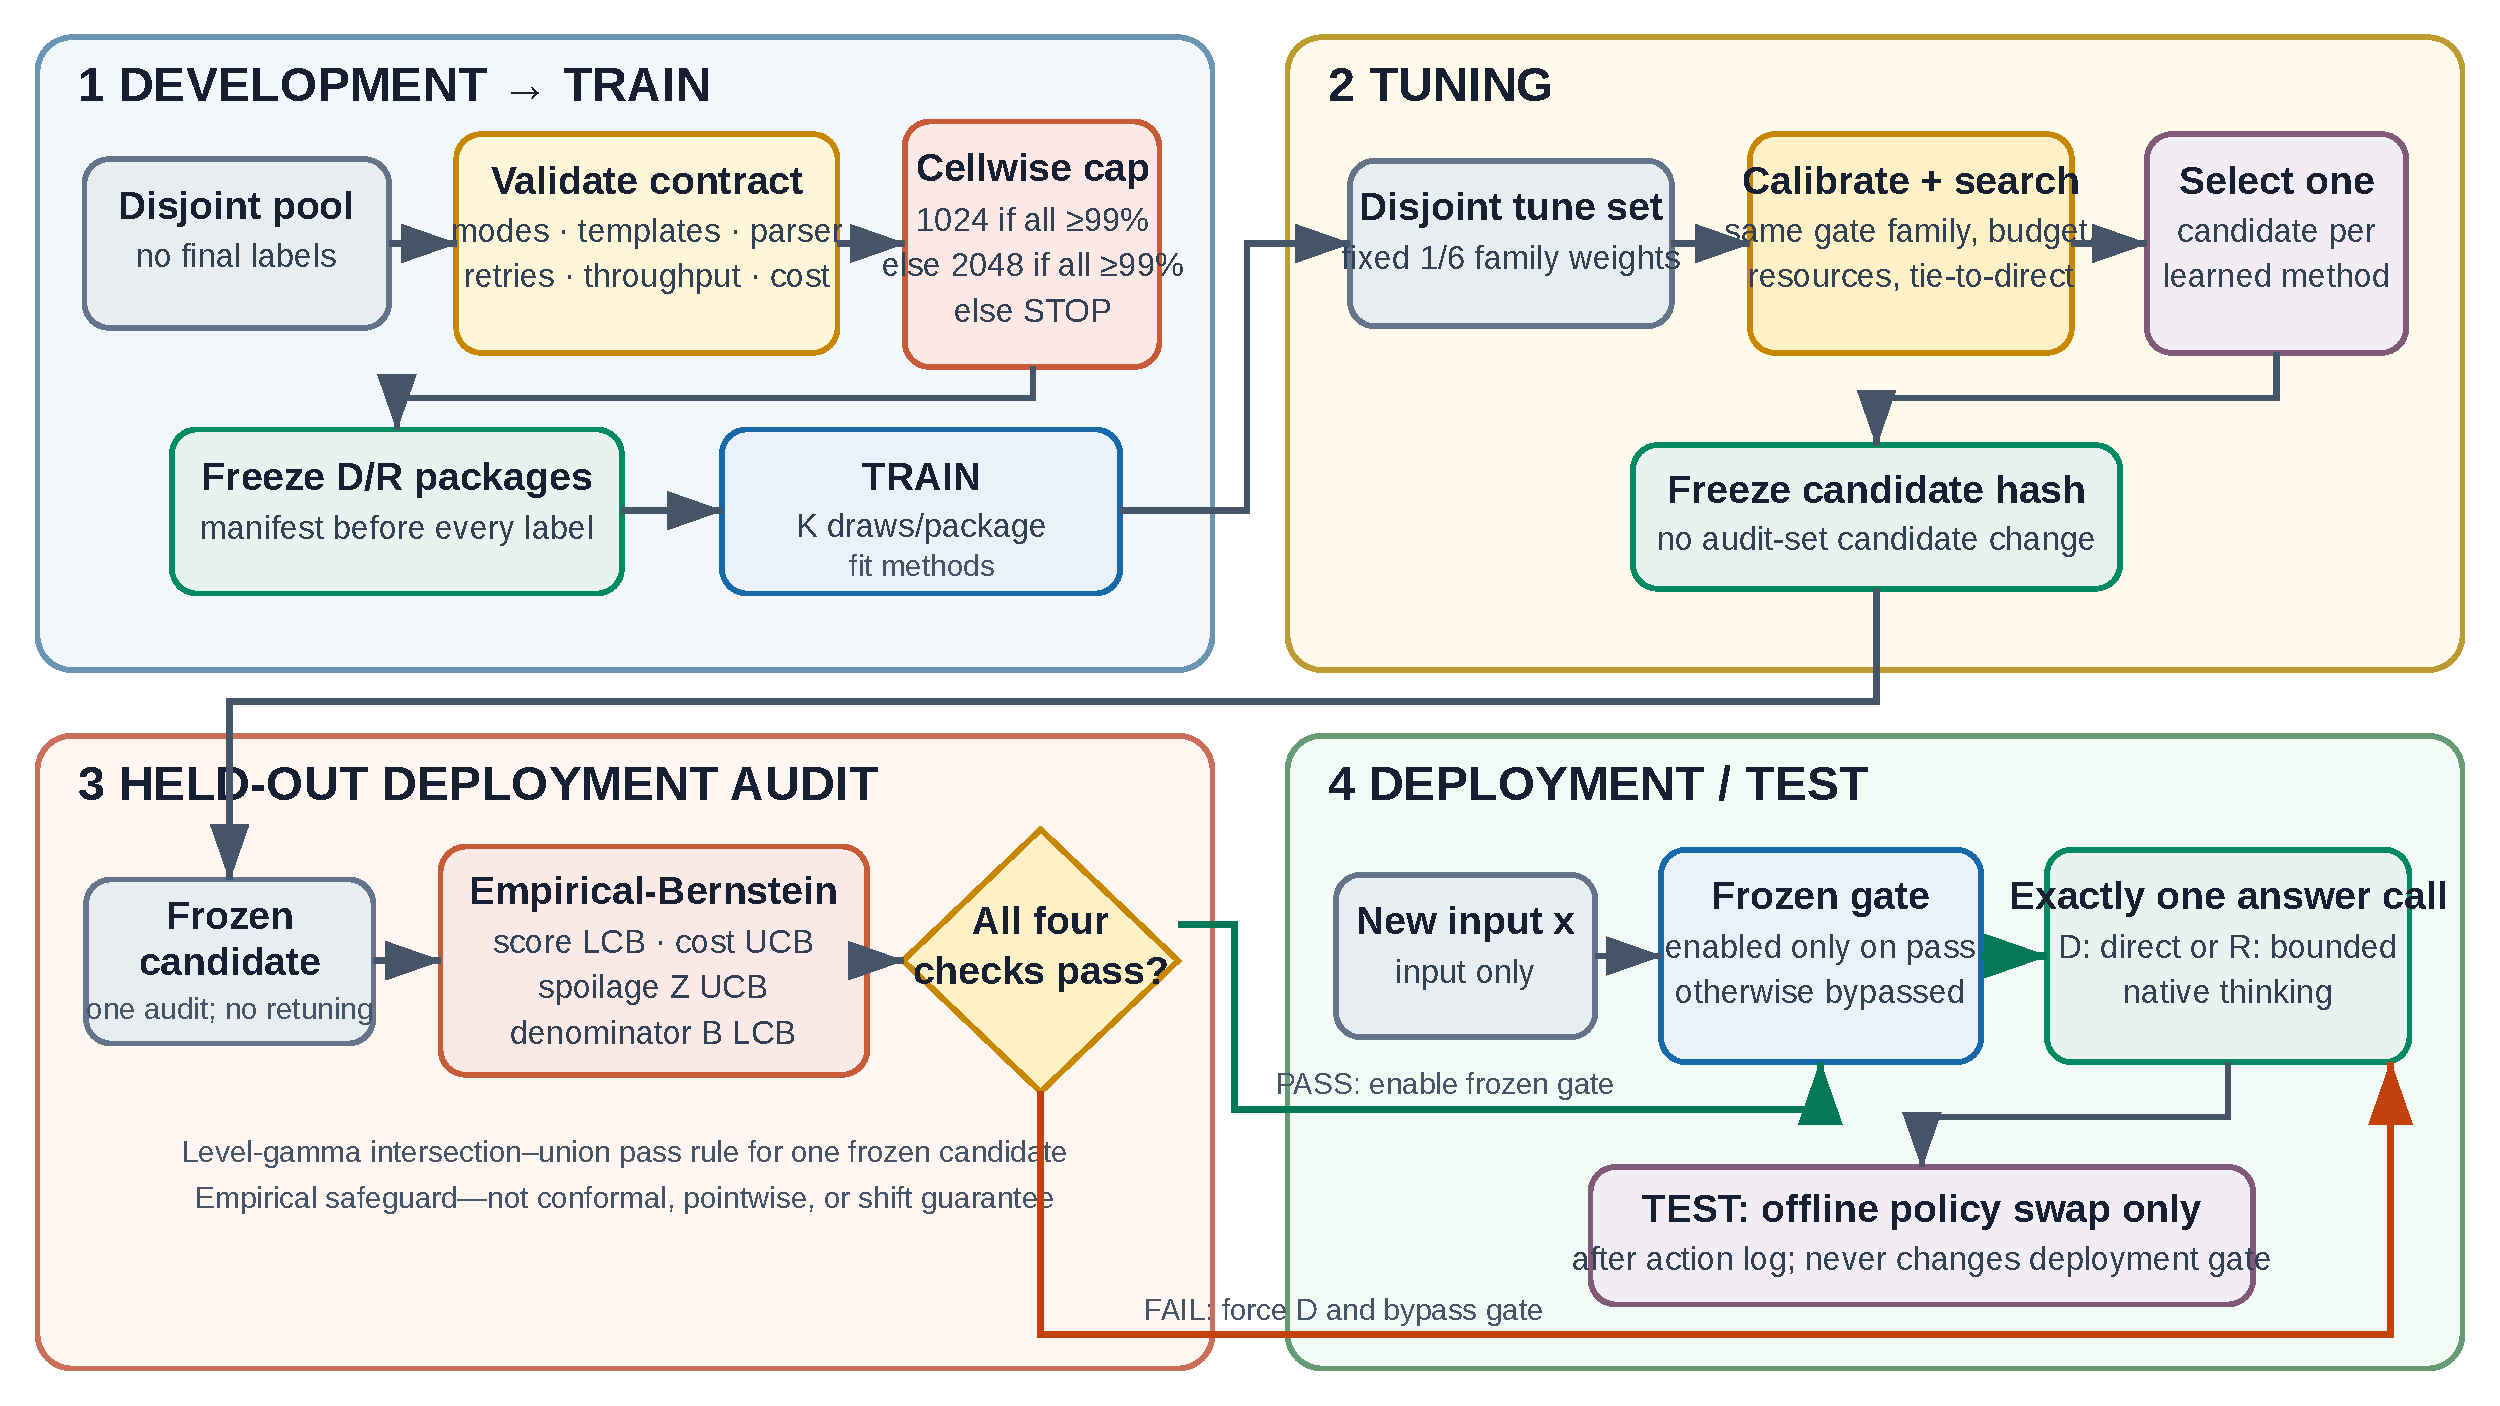
\includegraphics[width=\linewidth]{figures/taskcognition_architecture_critique_revised.pdf}
 \caption{\textbf{Frozen protocol and one-call deployment.} DEVELOPMENT precedes TRAIN and freezes both packages before any final rollout label. TUNING selects one candidate per learned method. A held-out empirical-Bernstein audit checks score, cost, spoilage, and denominator adequacy without retuning; failure forces \D{} and bypasses the gate. Deployment makes exactly one answer call. Test-time policy swap runs both packages offline only after the chosen action is logged and never changes the deployment gate.}
 \label{fig:architecture}
\end{figure}

A frozen encoder maps input text to an embedding, concatenated with cheap input-only observables such as length, numeric-token count, symbolic-operator count, multiple-choice markers, and format indicators. Dataset identity, latent generator parameters, answers, traces, verifier feedback, and direct drafts are prohibited. One shared-trunk multilayer perceptron predicts
$b_\phi(x)\approx\E[S_\Rpol-S_\D\mid X=x]$ and $q_\phi(x)\approx\hInd(x)$.

The benefit target is $T_{b,i}=\bar S_{\Rpol i}-\bar S_{\D i}$, trained primarily by the squared loss $(b_\phi(X_i)-T_{b,i})^2$, which elicits its conditional mean. A Huber loss is sensitivity-only. The harm head uses one soft-label log loss per instance,
\begin{equation}
 -T_{h,i}\log q_\phi(X_i)-(1-T_{h,i})\log\{1-q_\phi(X_i)\},
 \quad T_{h,i}=\widehat p_{\D i}(1-\widehat p_{\Rpol i}).
 \label{eq:harm-loss}
\end{equation}
This proper fractional-label objective \citep{gneiting2007strictly} is unweighted except for outcome-independent family or instance weights frozen before labels. It does not manufacture $K^2$ independent samples.

On TUNE, calibration maps, architecture, initialization, and thresholds are selected. The restricted gate is
\begin{equation}
 g_{\tau,\eta}(x)=\1\{\widetilde b_\phi(x)>\tau\ \land\ \widetilde q_\phi(x)\leq\eta\}.
 \label{eq:gate}
\end{equation}
Ties go to direct after the common score, cost, spoilage, and routing-rate tie-break order is frozen. The $q$ threshold is a restricted local joint-harm screen. It is not pointwise conditional spoilage, which would be $1-p_\Rpol(x)$ when $p_\D(x)>0$, and it is not a proof that Eq.~\ref{eq:objective} is globally optimized. Only the aggregate audit can authorize deployment.

\section{Development and Frozen Answer Contract}
The active TeX and \texttt{PROTOCOL\_SOURCE\_OF\_TRUTH.md} govern the current draft. Before any final label, a dated, hash-bound frozen manifest must become the sole executable specification. That manifest binds the model/tokenizer revision, engine/API invocation and chat-template hashes, precision, hardware, serialized prompts, samplers, cap, stop behavior, parsers, scorers, features, split and latent-ID manifests, $K$, $\alpha$, $\beta$, $b_{\min}$, $\delta_{\rm score}$, audit level, RNG streams, retry/timeout policy, cost schedule, candidate hashes, and direct fallback. A package change after freeze invalidates every rollout-derived label.

\paragraph{Development before labels.}
A separate six-family DEVELOPMENT pool is disjoint from all final rolls. It validates Qwen mode controls and templates, parsers and native adapters, pre-admission retry behavior, timeout handling, throughput, scalar cost accounting, cap feasibility, and sample/repeat allocation. It also supplies development reference charges and full-pipeline simulations, but no development rollout enters TRAIN, TUNE, AUDIT, or TEST.

The cellwise terminal cap rule is fixed. Package cap 1,024 is used only if every mode-by-family strict-valid-FINAL rate is at least 99\% in development. Otherwise 2,048 is used only if every cell reaches 99\%. If any cell remains below 99\%, the confirmatory study stops as infeasible for the bounded package. A larger cap may be studied only as a development diagnostic; Qwen's recommended long allowances are not the primary package. This rule is assessed before final labels, not on training completion curves.

\paragraph{Exactly two packages.}
Both packages use the same frozen \texttt{Qwen/Qwen3-8B} checkpoint and task information, no tools or feedback, and exactly one admitted answer generation \citep{yang2025qwen3,qwen3modelcard2026}. Package \D{} sets \texttt{enable\_thinking=False}; package \Rpol{} sets \texttt{enable\_thinking=True} with the frozen bounded cap. The primary matching sampler is sampling enabled, temperature $0.6$, top-$p$ $0.95$, top-$k$ $20$, and min-$p$ $0$ for both. The package-faithful sensitivity uses the model-card direct settings $(0.7,0.8,20,0)$ and reasoning settings $(0.6,0.95,20,0)$ for (temperature, top-$p$, top-$k$, min-$p$). The manifest pins the exact engine/API invocation that implements \texttt{enable\_thinking}, the chat template, and raw serialized prompts/completions.

\paragraph{Parser, retry, and failure contract.}
The strict sequence is: (i) native-think channelization; (ii) exactly one nonempty case-sensitive \texttt{<FINAL>} pair validated on the final channel, with no trailing text; and (iii) a version-pinned suite-native adapter and scorer. A FINAL-like tag in a reasoning trace is never authoritative. Status records distinguish native-delimiter failure, outer-wrapper failure, native-syntax failure, cap-without-final, valid partial credit, completed-native-wrong, and admitted execution/response failure.

Each draw permits one admitted answer generation. Deadline $T$, maximum pre-admission retries $J$, and RNG stream are frozen. A retry is allowed only when logs establish that no generation was admitted, using the identical request and stream; every dispatched attempt is charged. Unknown admission is treated as admitted. An admitted missing response, timeout, transport loss, malformed output, or cap stop is not retried and scores zero when no retainable valid response exists. In particular, an \Rpol{} runtime failure never triggers a direct answer. Thus deployment still contains two packages, one input-only gate, and one answer call.

\section{Comparators and Experimental Design}
\paragraph{Equally resourced learned comparators.}
Every learned method receives the same input information, frozen features, rollout table, split roles, overall trainable-parameter budget (within a disclosed prespecified tolerance), optimizer/search budget, calibration opportunities, tuning objective, family weights, tie-to-direct rule, all-in accounting, one frozen candidate, audit, and direct fallback. The \emph{winner router} uses $W_i=\1\{\bar S_{\Rpol i}>\bar S_{\D i}\}$, with exact ties assigned to direct. It fits a calibrated score $r_W(x)\approx\Prb(W=1\mid x)$ with one binary log loss per input and deploys $g^W_\tau(x)=\1\{\widetilde r_W(x)>\tau\}$. Its single threshold $\tau$ is tuned under the same $\Ew$ score/cost/spoilage objective and frozen tie-breaks. This is a winner-only gate family, not the two-head \TC{} family; resource parity, candidate selection, audit, and fallback are matched.

The \emph{factorized outcome router} predicts
\begin{equation}
 p_\D(x),\ p_\Rpol(x),\ \mu_\D(x)=\E[S_\D\mid x],\ \mu_\Rpol(x)=\E[S_\Rpol\mid x],
 \label{eq:factorized}
\end{equation}
and forms $b_F=\mu_\Rpol-\mu_\D$ and $h_F=p_\D(1-p_\Rpol)$. Fractional-label proper losses fit $p_a$ and squared losses fit $\mu_a$; binary families may share numerically identical outputs, while partial-credit families require both. It predicts cost only if a separately declared decision rule uses that prediction. \TC{} claims no information advantage over this factorization because its targets are algebraically recoverable. The empirical hypothesis is only a possible finite-data, calibration, or shift advantage from direct target learning.

Always-direct, always-reasoning, fixed random allocation, and observable-count thresholds are descriptive references. A nondeployable family-only allocation reference measures whether gains exceed coarse family allocation, but family ID remains prohibited at deployment. The \emph{same-rollout empirical oracle (optimistic under stochastic finite-$K$ selection)} is a descriptive ceiling with finite-$K$ selection bias; it is excluded from claims. No cascade appears in the primary table.

\paragraph{Splits and provisional counts.}
The confirmatory universe is the original-renderer Reasoning Gym version and six prespecified families: \texttt{number\_sorting}, \texttt{number\_format}, \texttt{letter\_counting}, \texttt{graph\_color}, \texttt{shortest\_path}, and \texttt{knights\_knaves} \citep{stojanovski2025reasoninggym,reasoninggymsoftware2026}. Current planning placeholders per family are 200 TRAIN, 75 TUNE, $n_f=n/6$ AUDIT, and 100 TEST inputs, with disjoint seeds. They are not evidence and will be finalized by development before final labels. Equal $1/6$ weighting defines a finite-family target, not a natural deployment distribution.

Renderer variants are paired only when generated from the same held-out latent problem ID and kept in the same split. Otherwise they are labeled unpaired fixed-case descriptions, with no renderer-effect attribution. LLMThinkBench remains separate test-only descriptive evidence \citep{srivastava-etal-2026-llms,llmthinkbenchsoftware2026}. The Mind-Your-Step-inspired set is independently generated new diagnostic material, not redistributed data or a replication \citep{pmlr-v267-liu25t,mindyourstepsoftware2025,taskcognitiondiagnosticplan2026}. Its generator/version and construct-validation criteria are frozen before final diagnostic generation; failed validation yields only a new procedural diagnostic label.

\section{Held-Out Deployment Audit}
Each of the six families contributes the same $n_f=n/6$ complete input clusters; development selects balanced $n$ before final labels. Latent problem IDs are independently sampled within family, RNG streams are independent by input and package, and failed rows are retained rather than dropped. Shared batch or system-failure units are eliminated or, if unavoidable, become the resampling and audit cluster. For the one tune-frozen candidate of a learned method, define cluster rows
\begin{align}
 B_i&=g_i\widehat p_{\D i}, &
 Z_i&=g_i\widehat p_{\D i}(1-\widehat p_{\Rpol i}-\alpha),\\
 \Delta_i&=g_i(\bar S_{\Rpol i}-\bar S_{\D i}), &
 C_i&=C_{\mathrm{gate},i}+(1-g_i)\bar C_{\D i}+g_i\bar C_{\Rpol i}.
 \label{eq:audit-rows}
\end{align}
Here $\Ew[Z]=\Ew[B]\{\Rspoil(g)-\alpha\}$. Let $\bar T=n^{-1}\sum_iT_i$ and $s_T^2=(n-1)^{-1}\sum_i(T_i-\bar T)^2$. For a row bounded in frozen $[a,b]$, use the finite-sample empirical-Bernstein radius for independent, not necessarily identically distributed rows \citep{maurer2009empirical}
\begin{equation}
 r_{\rm EB}(T)=\sqrt{\frac{2s_T^2\ln(2/\gamma)}{n}}
 +\frac{7(b-a)\ln(2/\gamma)}{3(n-1)},\qquad \gamma=0.05.
 \label{eq:eb}
\end{equation}
The declared ranges are $[-\alpha,1-\alpha]$ for $Z$, $[0,1]$ for $B$, $[-1,1]$ for $\Delta$, and development-frozen $[c_{\min},c_{\max}]$ for $C$. The latter is an analytic hard support bound derived from maximum input length, cap, retry ceiling, and the frozen tariff or service-time rule; it is not estimated from observed development extrema. A deterministic algebraic design calculation under normalized midpoint cost shows that the symmetric Hoeffding construction \citep{hoeffding1963probability} cannot jointly pass its cost and spoilage margins at the initial $n=450$ even in a favorable zero-spoilage idealization. This is not a TaskCognition feasibility run or result; $n=450$ is therefore not claimed sufficient. The empirical-Bernstein rule is frozen only after prospective validation over the full development simulation.

The candidate is enabled only if all four conditions hold:
\begin{equation}
 \bar Z+r_{\rm EB}(Z)\leq0,\quad
 \bar C+r_{\rm EB}(C)\leq\beta,\quad
 \bar B-r_{\rm EB}(B)\geq b_{\min}>0,\quad
 \bar\Delta-r_{\rm EB}(\Delta)\geq0.
 \label{eq:audit-pass}
\end{equation}
The first is a linearized aggregate spoilage check; the third enforces denominator precision; the fourth is score noninferiority, not superiority. Development full-pipeline simulation freezes $n$, $K$, $b_{\min}$, cost bounds, $\alpha$, and $\beta$. Audit data cannot change a candidate, threshold, or design quantity. Every learned method is audited separately and deploys direct if any check fails.

Equation~\ref{eq:audit-pass} is a level-$\gamma$ intersection--union pass rule for one frozen candidate under the declared independent-cluster design \citep{berger1996bioequivalence}. Because passage requires rejection of every component null, no Bonferroni adjustment is applied; the displayed bounds are not advertised as a joint confidence region. This empirical acceptance test is a deployment safeguard, not a novel certificate. It is not conformal, pointwise, distribution-free, or a renderer/suite-shift guarantee. Cluster bootstrap intervals may be reported descriptively only \citep{field2007bootstrapping}; test superiority is separate.

Adequacy reporting separates selected input count, weighted routing rate, $\bar B$ and its lower bound, raw nested direct successes $K\sum_i g_i\widehat p_{\D i}$, and Kish concentration $(\sum_i a_i)^2/\sum_i a_i^2$ for $a_i=n^{-1}g_i\widehat p_{\D i}$. Kish measures weight concentration, not ``effective direct-correct instances.''

\section{Primary Test, Planning, and Reporting}
For $m\in\{\text{always-direct},\text{winner},\text{factorized}\}$, define the original-renderer test contrast
\begin{equation}
 \Delta_m=\frac16\sum_{f=1}^6
 \overline{S_{\mathrm{TC,deploy}}-S_{m,\mathrm{deploy}}}^{\,(f)}.
 \label{eq:primary}
\end{equation}
Each learned comparator is its own audit-selected deployment: its frozen candidate if it passes, direct otherwise. Pre-audit candidate behavior is descriptive. The confirmatory contribution requires one-sided 95\% family-stratified paired instance-cluster bootstrap lower bounds above a development-frozen $\delta_{\rm score}\geq0$ for \emph{all three} contrasts. The manifest fixes the percentile interval construction, 10,000 within-family complete-cluster resamples, RNG seed, score aggregation over the $K$ draws, and failure handling before test access; a failed resample is retained with its frozen zero-score rule rather than redrawn. This bootstrap is asymptotic conditional on frozen deployments, not an exact randomization test. Whole input clusters are resampled within family, preserving equal family weights \citep{field2007bootstrapping}. This conjunctive claim does not use Holm correction; separately declared nonprimary families do. No sign-flip test is claimed exact.

Before any final label, a disjoint high-repeat development pool and full TRAIN$\rightarrow$TUNE$\rightarrow$AUDIT$\rightarrow$TEST simulation select balanced $n$, $b_{\min}$, $K$, and feasible $\alpha/\beta$ values. Each replicate fits and tunes each method, freezes one candidate, applies one audit, falls back to direct on failure, and evaluates the resulting deployment. Planned outputs include enablement, useful-candidate enablement, unsafe-candidate false enablement, fallback, bound widths, and conditional and unconditional test power or minimum detectable effect. A provisional high-repeat design is 25 inputs per family and 50 draws per package; this and all split counts are placeholders until DEVELOPMENT. These simulations are planning, not reported TaskCognition results or a promise of feasibility.

\begin{table}[t]
\caption{Primary test reporting contract. Every result cell is intentionally empty. Each learned row denotes its audit-selected deployment.}
\label{tab:primary}
\centering\small
\begin{tabular}{lccccc}
\toprule
Method & Score & $\Rspoil$ & $R_{DD}$ & R rate & Scalar cost \\
\midrule
Always direct & \NA & \NA & \NA & \NA & \NA \\
Always reasoning & \NA & \NA & \NA & \NA & \NA \\
Winner deployment & \NA & \NA & \NA & \NA & \NA \\
Factorized deployment & \NA & \NA & \NA & \NA & \NA \\
Family-only reference & \NA & \NA & \NA & \NA & \NA \\
\TC{} deployment & \NA & \NA & \NA & \NA & \NA \\
\bottomrule
\end{tabular}
\end{table}

\begin{table}[t]
\caption{Held-out audit contract for every learned method. All result fields, including hashes and decisions, remain empty until execution.}
\label{tab:audit}
\centering\scriptsize
\resizebox{\linewidth}{!}{%
\begin{tabular}{lcccccccccc}
\toprule
Method & Hash & $\bar B$ & $L_B$ & $\bar Z$ & $U_Z$ & $\bar C$ & $U_C$ & $\bar\Delta$ / $L_\Delta$ & Decision & Fallback \\
\midrule
Winner & \NA & \NA & \NA & \NA & \NA & \NA & \NA & \NA & \NA & \NA \\
Factorized & \NA & \NA & \NA & \NA & \NA & \NA & \NA & \NA & \NA & \NA \\
\TC{} & \NA & \NA & \NA & \NA & \NA & \NA & \NA & \NA & \NA & \NA \\
\bottomrule
\end{tabular}}
\end{table}

\section{Limitations and Conclusion}
The study concerns one checkpoint, two package distributions, one cap rule, fixed scorers, and a finite six-family target. Independent-draw spoilage is not a causal switch; finite $K$ yields noisy input targets; and $d_\epsilon$ and expected score capture losses omitted by perfect correctness. An aggregate audit can miss family heterogeneity and cannot transfer to renderer or external-suite shift. Empirical-Bernstein validity depends on the frozen bounded ledger and independent complete clusters. Renderer cases not paired by latent ID remain unpaired descriptions. The same-rollout empirical oracle is optimistic. No non-significant contrast will be called equivalence.

\TC{} asks whether paired benefit and independent-draw spoilage supervision improves a constrained choice between \D{} and \Rpol{} beyond same-resource winner and factorized outcome routers. Package freeze precedes labels; tuning selects once; each method is audited once; failure forces direct; and test superiority is adjudicated separately. No TaskCognition result, audit passage, power estimate, or novel effect is reported in this manuscript.

\subsection*{Reproducibility statement}
The active manuscript plus the governed dated manifest will be the sole implementation specification. Before test access, the release will archive immutable hashes for packages, prompts, parsers, features, data splits, candidates, audit code, cost schedule, random streams, and fallback. Historical conflicting notes remain marked superseded. Outputs will be released only where licenses permit; otherwise permitted identifiers, hashes, derived cluster rows, and evaluation code will be provided.

\subsection*{AI use statement (draft stage)}
Generative AI assisted literature organization, critique-driven protocol revision, prose editing, BibTeX preparation, and vector figure layout. It did not execute TaskCognition experiments or generate evidence. Authors must verify every source, protocol component, artifact, and claim before submission and retain responsibility for the final work.

\clearpage
\bibliography{taskcognition}
\bibliographystyle{iclr2027_conference}

\appendix
\section{Frozen Protocol Details}
\subsection{Stage and manifest contract}
The final manifest is created only after DEVELOPMENT. If any package-defining element changes thereafter, all TRAIN, TUNE, AUDIT, and TEST rollout-derived labels are regenerated. The executable order is:
\begin{verbatim}
DEVELOPMENT (disjoint): validate modes, templates, parsers,
  retries, throughput, and one scalar ledger; apply the
  cellwise cap rule; run high-repeat and full-pipeline
  design simulations; freeze the manifest.
TRAIN: collect K draws from both frozen packages;
  aggregate one row per input;
  fit winner, factorized, and TaskCognition methods.
TUNE: calibrate/search with E_w; freeze one candidate and
  hash per method.
AUDIT: apply each candidate once; compute empirical-
  Bernstein B/Z/C/Delta
  checks; on any failure deploy direct. Never retune on audit.
TEST: evaluate frozen deployments; force D and R offline
  only after the selected action is logged; never update
  a gate.
\end{verbatim}

\subsection{Planned sample manifest}
Table~\ref{tab:manifest} contains provisional design placeholders, not results. Development may change them before final labels; after the manifest is frozen, test access cannot.
\begin{table}[t]
\caption{Provisional balanced counts to be finalized by development simulation.}
\label{tab:manifest}
\centering\small
\begin{tabular}{lrrrrr}
\toprule
Source & Development & Train & Tune & Audit & Test \\
\midrule
Reasoning Gym, per family & TBD & 200 & 75 & $n/6$ & 100 \\
Reasoning Gym, six families & TBD & 1200 & 450 & $n$ & 600 \\
LLMThinkBench & 0 & 0 & 0 & 0 & descriptive \\
Independent diagnostic & TBD & 0 & 0 & 0 & descriptive \\
\bottomrule
\end{tabular}
\end{table}

\subsection{Audit implementation and descriptive bootstrap}
For each method, analysis verifies the candidate hash and complete balanced family membership, computes Eq.~\ref{eq:audit-rows} from one row per input, checks the frozen ranges, and evaluates Eq.~\ref{eq:audit-pass} without candidate search. The all-in cost bound includes the gate and all dispatched attempts. A missing, failed, or mismatched audit artifact invokes direct deployment.

Any descriptive bootstrap resamples complete inputs within each family, recomputes $\Ew$ and every ratio inside the replicate, and uses a frozen replicate count, seed, interval rule, and zero-denominator convention. Such intervals do not determine deployment. Package-output reports are mode-by-family and separate admitted generations, pre-admission retries, transport/timeouts, finish reason, cap-without-final, native-delimiter errors, outer-wrapper errors, native-syntax errors, valid partial credit, completed wrong answers, and successes.

\begin{table}[t]
\caption{Planned learned-method adequacy report; all result cells are empty.}
\centering\scriptsize
\begin{tabular}{lcccccc}
\toprule
Method & Selected $N$ & Weighted route & $\bar B/L_B$ & Raw nested successes & Kish & Audit action \\
\midrule
Winner & \NA & \NA & \NA & \NA & \NA & \NA \\
Factorized & \NA & \NA & \NA & \NA & \NA & \NA \\
\TC{} & \NA & \NA & \NA & \NA & \NA & \NA \\
\bottomrule
\end{tabular}
\end{table}

\begin{table}[t]
\caption{Planned package quality-control report, stratified by the two modes and six families; all cells are empty.}
\centering\scriptsize
\begin{tabular}{lcccccc}
\toprule
Mode--family cell & Admitted $N$ & Valid FINAL & Cap/no final & Native delimiter & Wrapper/syntax & Partial/wrong \\
\midrule
Direct, six cells & \NA & \NA & \NA & \NA & \NA & \NA \\
Reasoning, six cells & \NA & \NA & \NA & \NA & \NA & \NA \\
\bottomrule
\end{tabular}
\end{table}

\section{Secondary Analyses and Interpretive Boundaries}
Per-family score, cost, routing, $\Rspoil$, direct-success mass, $R_{DD}$, $\Delta_{DD}$, and the three score contrasts will be reported descriptively. External suites and renderer variants never inherit the original-renderer audit. If latent-ID pairing is available, renderer comparisons resample latent-problem clusters; otherwise only separate fixed-case values are shown.

A future cascade analysis must retain each direct preview jointly with its confidence and correctness, charge that preview and all escalation work, and define a preview-conditional risk such as
\[
 \frac{\E[eY_{\D0}(1-Y_{\Rpol1})]}{\E[eY_{\D0}]},
\]
where $e$ may observe $(X,Y_{\D0})$ and $Y_{\Rpol1}$ is an independent reasoning draw. It is not numerically interchangeable with Eq.~\ref{eq:rspoil} and cannot be inserted into the primary table. Cost-aware Lagrangians, per-query bounds, additional checkpoints, tools, agents, and new policy checkpoints likewise require separate protocols.

\section{Pre-Execution Checklist}
Before final rollouts, the authors will verify: six-family development coverage; Qwen mode separation; serialized template hashes; strict parser order; terminal cap decision; the retry/admission state machine; one scalar cost schedule and hard bounds; high-repeat target-variance estimates; full-pipeline false-enable and power simulations; frozen $K,n,b_{\min},\alpha,\beta,\delta_{\rm score}$; disjoint seed and latent-ID manifests; candidate-resource parity; and analysis unit tests. This checklist authorizes implementation only; it cannot be filled with post-test choices.

\end{document}
